

\tikzset{every picture/.style={line width=0.75pt}} %set default line width to 0.75pt        

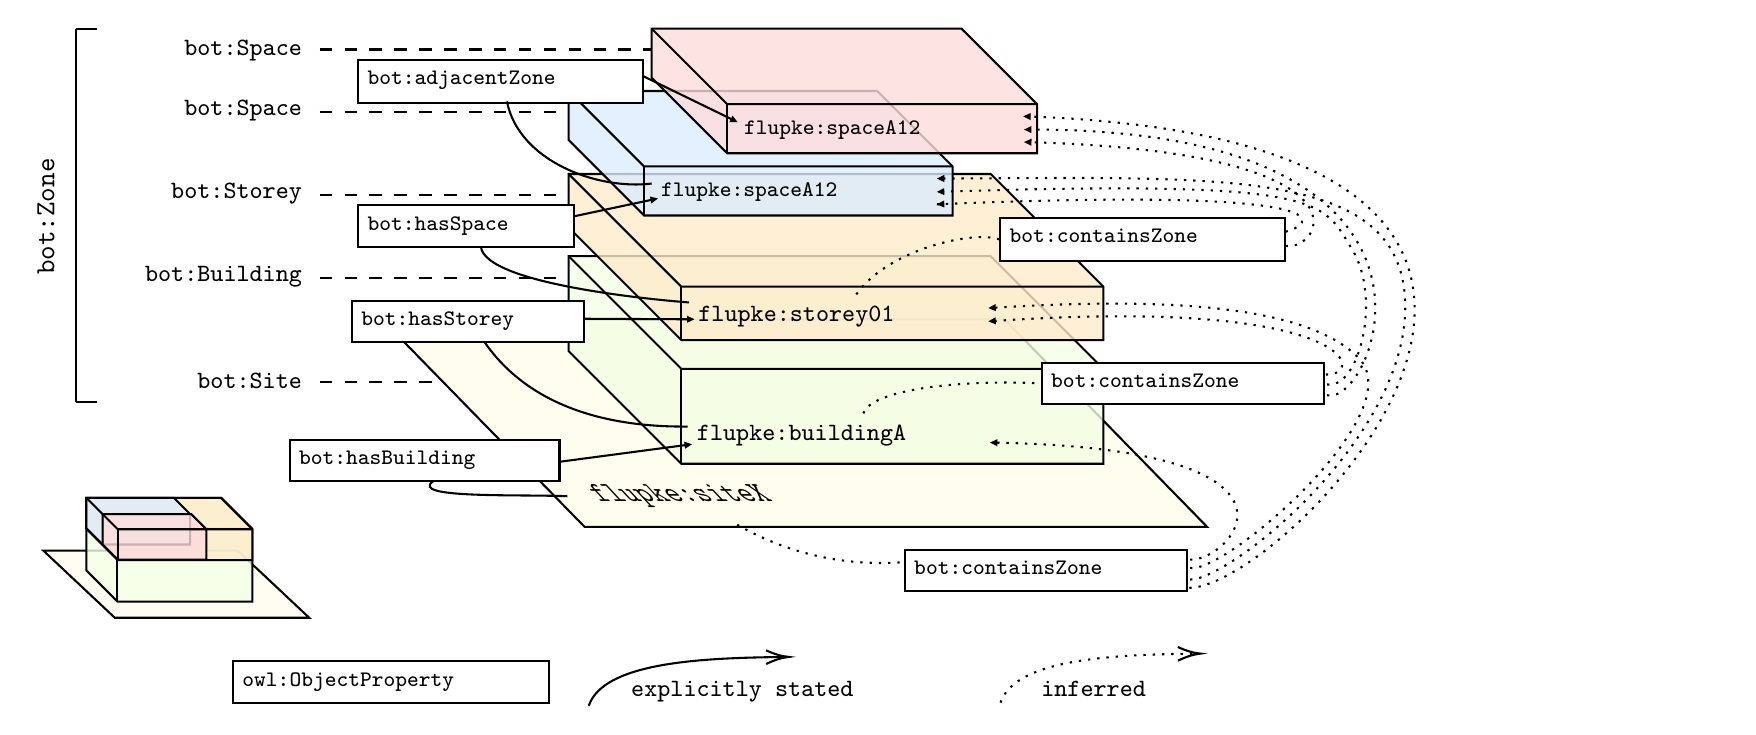
\begin{tikzpicture}[x=0.75pt,y=0.75pt,yscale=-1,xscale=1]
    \ttfamily
%uncomment if require: \path (0,373); %set diagram left start at 0, and has height of 373

%Shape: Parallelogram [id:dp6234888353745478] 
\draw  [fill={rgb, 255:red, 255; green, 253; blue, 237 }  ,fill opacity=0.8 ] (113,261.47) -- (19.33,261.47) -- (53.73,293.8) -- (147.4,293.8) -- cycle ;
%Shape: Parallelogram [id:dp5369889401184471] 
\draw  [fill={rgb, 255:red, 255; green, 253; blue, 237 }  ,fill opacity=1 ] (482.33,150) -- (182.41,150) -- (280.07,250) -- (580,250) -- cycle ;
%Shape: Cube [id:dp8255469967169493] 
\draw  [fill={rgb, 255:red, 243; green, 255; blue, 228 }  ,fill opacity=0.8 ] (530,173.85) -- (475.75,119.6) -- (272.41,119.6) -- (272.41,165.35) -- (326.66,219.6) -- (530,219.6) -- cycle ; \draw   (272.41,119.6) -- (326.66,173.85) -- (530,173.85) ; \draw   (326.66,173.85) -- (326.66,219.6) ;
%Shape: Cube [id:dp7451550676115966] 
\draw  [fill={rgb, 255:red, 254; green, 235; blue, 202 }  ,fill opacity=0.8 ] (530,134.25) -- (475.75,80) -- (272.41,80) -- (272.41,105.75) -- (326.66,160) -- (530,160) -- cycle ; \draw   (272.41,80) -- (326.66,134.25) -- (530,134.25) ; \draw   (326.66,134.25) -- (326.66,160) ;
%Shape: Cube [id:dp7376474366082748] 
\draw  [fill={rgb, 255:red, 220; green, 236; blue, 254 }  ,fill opacity=0.8 ] (457.41,76.33) -- (421.07,40) -- (272.41,40) -- (272.41,63.67) -- (308.74,100) -- (457.41,100) -- cycle ; \draw   (272.41,40) -- (308.74,76.33) -- (457.41,76.33) ; \draw   (308.74,76.33) -- (308.74,100) ;
%Shape: Cube [id:dp6037678452495017] 
\draw  [fill={rgb, 255:red, 254; green, 220; blue, 220 }  ,fill opacity=0.8 ][line width=0.75]  (498.07,46.33) -- (461.74,10) -- (312.41,10) -- (312.41,33.67) -- (348.74,70) -- (498.07,70) -- cycle ; \draw  [line width=0.75]  (312.41,10) -- (348.74,46.33) -- (498.07,46.33) ; \draw  [line width=0.75]  (348.74,46.33) -- (348.74,70) ;
%Curve Lines [id:da34503747339894364] 
\draw  [dash pattern={on 0.84pt off 2.51pt}]  (617.81,114.6) .. controls (634.52,117.78) and (665.49,69.49) .. (494.4,64.67) ;
\draw [shift={(491.81,64.6)}, rotate = 1.45] [fill={rgb, 255:red, 0; green, 0; blue, 0 }  ][line width=0.08]  [draw opacity=0] (3.57,-1.72) -- (0,0) -- (3.57,1.72) -- cycle    ;
%Curve Lines [id:da8352390399084118] 
\draw  [dash pattern={on 0.84pt off 2.51pt}]  (617.81,107.8) .. controls (628.61,105.4) and (659.41,85.8) .. (449.81,94.6) ;
\draw [shift={(449.81,94.6)}, rotate = 357.6] [fill={rgb, 255:red, 0; green, 0; blue, 0 }  ][line width=0.08]  [draw opacity=0] (3.57,-1.72) -- (0,0) -- (3.57,1.72) -- cycle    ;
%Curve Lines [id:da4764695659197302] 
\draw  [dash pattern={on 0.84pt off 2.51pt}]  (637.81,186.6) .. controls (660.61,192.6) and (716.61,57) .. (491.81,58.6) ;
\draw [shift={(491.81,58.6)}, rotate = 359.59] [fill={rgb, 255:red, 0; green, 0; blue, 0 }  ][line width=0.08]  [draw opacity=0] (3.57,-1.72) -- (0,0) -- (3.57,1.72) -- cycle    ;
%Curve Lines [id:da6997716856913325] 
\draw  [dash pattern={on 0.84pt off 2.51pt}]  (637.81,181.4) .. controls (653.41,183.8) and (664.21,139.4) .. (649.81,116.2) .. controls (635.48,93.12) and (638.97,82.7) .. (452.63,88.51) ;
\draw [shift={(449.81,88.6)}, rotate = 358.18] [fill={rgb, 255:red, 0; green, 0; blue, 0 }  ][line width=0.08]  [draw opacity=0] (3.57,-1.72) -- (0,0) -- (3.57,1.72) -- cycle    ;
%Curve Lines [id:da2611543315656344] 
\draw  [dash pattern={on 0.84pt off 2.51pt}]  (637.21,176.6) .. controls (656.91,177.4) and (651.86,138.99) .. (477.25,150.82) ;
\draw [shift={(474.61,151)}, rotate = 356] [fill={rgb, 255:red, 0; green, 0; blue, 0 }  ][line width=0.08]  [draw opacity=0] (3.57,-1.72) -- (0,0) -- (3.57,1.72) -- cycle    ;
%Curve Lines [id:da3444743375210677] 
\draw  [dash pattern={on 0.84pt off 2.51pt}]  (571.41,279.4) .. controls (618.61,279.4) and (830.21,63.4) .. (491.41,52.2) ;
\draw [shift={(491.41,52.2)}, rotate = 1.89] [fill={rgb, 255:red, 0; green, 0; blue, 0 }  ][line width=0.08]  [draw opacity=0] (3.57,-1.72) -- (0,0) -- (3.57,1.72) -- cycle    ;
%Curve Lines [id:da00012227444950441146] 
\draw  [dash pattern={on 0.84pt off 2.51pt}]  (571.81,269.8) .. controls (588.81,272.6) and (679.01,195) .. (653.01,168.6) .. controls (627.27,142.46) and (556.83,139.46) .. (477.03,144.45) ;
\draw [shift={(474.61,144.6)}, rotate = 356.32] [fill={rgb, 255:red, 0; green, 0; blue, 0 }  ][line width=0.08]  [draw opacity=0] (3.57,-1.72) -- (0,0) -- (3.57,1.72) -- cycle    ;
%Curve Lines [id:da2737876317435528] 
\draw  [dash pattern={on 0.84pt off 2.51pt}]  (571.81,265.8) .. controls (591.51,266.6) and (641.3,212.35) .. (477.89,209.44) ;
\draw [shift={(475.41,209.4)}, rotate = 0.83] [fill={rgb, 255:red, 0; green, 0; blue, 0 }  ][line width=0.08]  [draw opacity=0] (3.57,-1.72) -- (0,0) -- (3.57,1.72) -- cycle    ;
%Curve Lines [id:da48651030268326223] 
\draw  [dash pattern={on 0.84pt off 2.51pt}]  (571.81,275.4) .. controls (591.47,275.4) and (678.21,205.8) .. (675.41,141) .. controls (672.62,76.52) and (587.07,81.75) .. (451.85,82.19) ;
\draw [shift={(449.81,82.2)}, rotate = 359.83] [fill={rgb, 255:red, 0; green, 0; blue, 0 }  ][line width=0.08]  [draw opacity=0] (3.57,-1.72) -- (0,0) -- (3.57,1.72) -- cycle    ;
%Straight Lines [id:da018272292431112502] 
\draw  [dash pattern={on 4.5pt off 4.5pt}]  (152.41,20) -- (312.41,20) ;
%Straight Lines [id:da7335835552603491] 
\draw  [dash pattern={on 4.5pt off 4.5pt}]  (152.41,50) -- (272.41,50) ;
%Straight Lines [id:da8480379890588858] 
\draw  [dash pattern={on 4.5pt off 4.5pt}]  (152.41,90) -- (272.41,90) ;
%Straight Lines [id:da5645617535440737] 
\draw  [dash pattern={on 4.5pt off 4.5pt}]  (152.41,130) -- (272.41,130) ;
%Straight Lines [id:da7578549164754749] 
\draw  [dash pattern={on 4.5pt off 4.5pt}]  (152.41,180) -- (212.41,180) ;
%Straight Lines [id:da4046157540132602] 
\draw    (35,10) -- (35,190) ;
%Straight Lines [id:da9585577369264056] 
\draw    (35,10) -- (45,10) ;
%Straight Lines [id:da8679205527736427] 
\draw    (35,190) -- (45,190) ;
%Straight Lines [id:da4346199951984231] 
\draw    (265.4,219) -- (328.83,210.59) ;
\draw [shift={(331.8,210.2)}, rotate = 172.45] [fill={rgb, 255:red, 0; green, 0; blue, 0 }  ][line width=0.08]  [draw opacity=0] (3.57,-1.72) -- (0,0) -- (3.57,1.72) -- cycle    ;
%Straight Lines [id:da9955272147380352] 
\draw    (275.7,149.72) -- (330,149.99) ;
\draw [shift={(333,150)}, rotate = 180.28] [fill={rgb, 255:red, 0; green, 0; blue, 0 }  ][line width=0.08]  [draw opacity=0] (3.57,-1.72) -- (0,0) -- (3.57,1.72) -- cycle    ;
%Straight Lines [id:da5290759611186164] 
\draw    (268.7,101.72) -- (312.47,92.42) ;
\draw [shift={(315.4,91.8)}, rotate = 168.01] [fill={rgb, 255:red, 0; green, 0; blue, 0 }  ][line width=0.08]  [draw opacity=0] (3.57,-1.72) -- (0,0) -- (3.57,1.72) -- cycle    ;
%Straight Lines [id:da2082247372760495] 
\draw    (307.8,32.6) -- (351.1,53.69) ;
\draw [shift={(353.8,55)}, rotate = 205.96] [fill={rgb, 255:red, 0; green, 0; blue, 0 }  ][line width=0.08]  [draw opacity=0] (3.57,-1.72) -- (0,0) -- (3.57,1.72) -- cycle    ;
%Shape: Cube [id:dp41271376617212563] 
\draw  [fill={rgb, 255:red, 243; green, 255; blue, 228 }  ,fill opacity=0.8 ] (120,251) -- (105,236) -- (40,236) -- (40,271) -- (55,286) -- (120,286) -- cycle ; \draw   (40,236) -- (55,251) -- (120,251) ; \draw   (55,251) -- (55,286) ;
%Shape: Cube [id:dp24709864473657217] 
\draw  [fill={rgb, 255:red, 254; green, 235; blue, 202 }  ,fill opacity=0.8 ] (120,251.17) -- (104.83,236) -- (40,236) -- (40,250.83) -- (55.17,266) -- (120,266) -- cycle ; \draw   (40,236) -- (55.17,251.17) -- (120,251.17) ; \draw   (55.17,251.17) -- (55.17,266) ;
%Shape: Cube [id:dp7279118293384432] 
\draw  [fill={rgb, 255:red, 220; green, 236; blue, 254 }  ,fill opacity=0.8 ] (90,243.83) -- (82.17,236) -- (40,236) -- (40,250.67) -- (47.83,258.5) -- (90,258.5) -- cycle ; \draw   (40,236) -- (47.83,243.83) -- (90,243.83) ; \draw   (47.83,243.83) -- (47.83,258.5) ;
%Shape: Cube [id:dp46117172286245767] 
\draw  [fill={rgb, 255:red, 254; green, 220; blue, 220 }  ,fill opacity=0.8 ] (97.83,251.17) -- (90.5,243.83) -- (47.83,243.83) -- (47.83,258.5) -- (55.17,265.83) -- (97.83,265.83) -- cycle ; \draw   (47.83,243.83) -- (55.17,251.17) -- (97.83,251.17) ; \draw   (55.17,251.17) -- (55.17,265.83) ;
%Curve Lines [id:da718845720785724] 
\draw    (282.08,336.27) .. controls (289.17,314.99) and (337.4,313.12) .. (376.69,312.69) ;
\draw [shift={(378.48,312.67)}, rotate = 179.42] [color={rgb, 255:red, 0; green, 0; blue, 0 }  ][line width=0.75]    (10.93,-3.29) .. controls (6.95,-1.4) and (3.31,-0.3) .. (0,0) .. controls (3.31,0.3) and (6.95,1.4) .. (10.93,3.29)   ;
%Curve Lines [id:da5183556614244442] 
\draw  [dash pattern={on 0.84pt off 2.51pt}]  (480.48,334.67) .. controls (487.57,313.39) and (535.8,311.52) .. (575.09,311.09) ;
\draw [shift={(576.88,311.07)}, rotate = 179.42] [color={rgb, 255:red, 0; green, 0; blue, 0 }  ][line width=0.75]    (10.93,-3.29) .. controls (6.95,-1.4) and (3.31,-0.3) .. (0,0) .. controls (3.31,0.3) and (6.95,1.4) .. (10.93,3.29)   ;

% Text Node
\draw (276.69,228) node [anchor=north west][inner sep=0.75pt]  [xslant=-0.93] [align=left] {flupke:siteX};
% Text Node
\draw (332.74,199.33) node [anchor=north west][inner sep=0.75pt]  [font=\small] [align=left] {flupke:buildingA \ \ \ \ \ \ \ \ \ \ };
% Text Node
\draw (333.41,142) node [anchor=north west][inner sep=0.75pt]  [font=\small] [align=left] {flupke:storey01 \ \ \ \ \ \ \ \ \ \ };
% Text Node
\draw (355.41,53) node [anchor=north west][inner sep=0.75pt]  [font=\footnotesize] [align=left] {flupke:spaceA12 \ \ \ \ \ \ \ \ \ \ };
% Text Node
\draw  [fill={rgb, 255:red, 255; green, 255; blue, 255 }  ,fill opacity=1 ]  (480.41,101) -- (617.41,101) -- (617.41,122) -- (480.41,122) -- cycle  ;
\draw (483.41,105) node [anchor=north west][inner sep=0.75pt]  [font=\footnotesize] [align=left] {bot:containsZone \ \ \ \ \ \ \ \ \ \ };
% Text Node
\draw  [fill={rgb, 255:red, 255; green, 255; blue, 255 }  ,fill opacity=1 ]  (500.41,171) -- (636.41,171) -- (636.41,191) -- (500.41,191) -- cycle  ;
\draw (503.41,175) node [anchor=north west][inner sep=0.75pt]  [font=\footnotesize] [align=left] {bot:containsZone \ \ \ \ \ \ \ \ \ \ };
% Text Node
\draw  [fill={rgb, 255:red, 255; green, 255; blue, 255 }  ,fill opacity=1 ]  (434.41,261) -- (570.41,261) -- (570.41,281) -- (434.41,281) -- cycle  ;
\draw (437.41,265) node [anchor=north west][inner sep=0.75pt]  [font=\footnotesize] [align=left] {bot:containsZone \ \ \ \ \ \ \ \ \ \ };
% Text Node
\draw (315.41,83) node [anchor=north west][inner sep=0.75pt]  [font=\footnotesize] [align=left] {flupke:spaceA12 \ \ \ \ \ \ \ \ \ \ };
% Text Node
\draw (145.41,20.5) node [anchor=east] [inner sep=0.75pt]  [font=\small] [align=left] {bot:Space};
% Text Node
\draw (145.41,49.5) node [anchor=east] [inner sep=0.75pt]  [font=\small] [align=left] {bot:Space};
% Text Node
\draw (145.41,89.5) node [anchor=east] [inner sep=0.75pt]  [font=\small] [align=left] {bot:Storey};
% Text Node
\draw (145.41,129.5) node [anchor=east] [inner sep=0.75pt]  [font=\small] [align=left] {bot:Building};
% Text Node
\draw (145.41,179.5) node [anchor=east] [inner sep=0.75pt]  [font=\small] [align=left] {bot:Site};
% Text Node
\draw (20.5,100.5) node  [font=\normalsize,rotate=-270] [align=left] {bot:Zone};
% Text Node
\draw  [fill={rgb, 255:red, 255; green, 255; blue, 255 }  ,fill opacity=1 ]  (138,208) -- (268,208) -- (268,228) -- (138,228) -- cycle  ;
\draw (141,212) node [anchor=north west][inner sep=0.75pt]  [font=\footnotesize] [align=left] {bot:hasBuilding \ \ \ \ \ \ \ \ \ \ \ };
% Text Node
\draw  [fill={rgb, 255:red, 255; green, 255; blue, 255 }  ,fill opacity=1 ]  (168,141) -- (280,141) -- (280,161) -- (168,161) -- cycle  ;
\draw (171,145) node [anchor=north west][inner sep=0.75pt]  [font=\footnotesize] [align=left] {bot:hasStorey \ \ \ \ \ \ \ \ };
% Text Node
\draw  [fill={rgb, 255:red, 255; green, 255; blue, 255 }  ,fill opacity=1 ]  (171,25) -- (308,25) -- (308,46) -- (171,46) -- cycle  ;
\draw (174,29) node [anchor=north west][inner sep=0.75pt]  [font=\footnotesize] [align=left] {bot:adjacentZone \ \ \ \ \ \ \ \ \ \ };
% Text Node
\draw  [fill={rgb, 255:red, 255; green, 255; blue, 255 }  ,fill opacity=1 ]  (171,95) -- (275,95) -- (275,115) -- (171,115) -- cycle  ;
\draw (174,99) node [anchor=north west][inner sep=0.75pt]  [font=\footnotesize] [align=left] {bot:hasSpace \ \ \ \ \ \ };
% Text Node
\draw  [fill={rgb, 255:red, 255; green, 255; blue, 255 }  ,fill opacity=1 ]  (110.74,314.83) -- (262.74,314.83) -- (262.74,334.83) -- (110.74,334.83) -- cycle  ;
\draw (113.74,318.83) node [anchor=north west][inner sep=0.75pt]  [font=\footnotesize] [align=left] {owl:ObjectProperty \ \ \ \ \ \ \ \ \ \ \ \ };
% Text Node
\draw (301.04,322.88) node [anchor=north west][inner sep=0.75pt]  [font=\small] [align=left] {explicitly stated};
% Text Node
\draw (498.64,322.88) node [anchor=north west][inner sep=0.75pt]  [font=\small] [align=left] {inferred};
% Connection
\draw  [dash pattern={on 0.84pt off 2.51pt}]  (353.59,249) .. controls (378.56,263.15) and (405.5,269.14) .. (434.41,266.98) ;
% Connection
\draw  [dash pattern={on 0.84pt off 2.51pt}]  (414.39,195.33) .. controls (417.83,184.2) and (459.52,178.83) .. (500.41,180.89) ;
% Connection
\draw  [dash pattern={on 0.84pt off 2.51pt}]  (411,138) .. controls (426.16,116.24) and (468.16,106.77) .. (480.41,111.68) ;
% Connection
\draw    (271.82,235.25) .. controls (248.39,234.24) and (195.05,236.49) .. (207.18,228) ;
% Connection
\draw    (329.74,201.67) .. controls (289.49,202.06) and (252.87,191.28) .. (231.88,161) ;
% Connection
\draw    (330.41,141.89) .. controls (315.58,140.78) and (232.01,133.24) .. (230.12,115) ;
% Connection
\draw    (312.41,84.59) .. controls (286.33,87.84) and (248.33,73.82) .. (242.66,45) ;

\end{tikzpicture}
